% =====================================================================
%  PRESENTATION TIPE - VERSION COMPLETE ET RIGOUREUSE
%  Modele poutre 1D + validation RLC. Ordres de grandeur chiffres.
%  Compilation : pdflatex presentation_complete.tex (x2).
%  Image motivation : fichier fc23c2280ceeb0d2edc34ce22218e61e-1540472534.jpg
%  (sinon un cadre de substitution s'affiche : le doc compile quand meme).
% =====================================================================
\documentclass[11pt,aspectratio=169]{beamer}
\usetheme{Madrid}\usecolortheme{whale}
\setbeamertemplate{navigation symbols}{}
\usepackage[utf8]{inputenc}
\usepackage[T1]{fontenc}
\usepackage[french]{babel}
\usepackage{amsmath,amssymb}
\usepackage{graphicx}
\usepackage{xcolor}
\usepackage{booktabs}
\usepackage{enumitem}
\usepackage{tikz}
\usetikzlibrary{arrows.meta,positioning,decorations.pathmorphing,
                patterns,shapes.geometric,calc}

\definecolor{verre}{RGB}{30,120,180}
\definecolor{danger}{RGB}{200,40,40}
\definecolor{ok}{RGB}{30,150,90}
\definecolor{gristik}{RGB}{120,120,120}

% --- sol hachure : \sol{xg}{xd} ---
\newcommand{\sol}[2]{%
  \draw[thick](#1,0)--(#2,0);
  \foreach \xx in {#1,...,#2}{\draw[gristik](\xx,0)--(\xx-0.25,-0.25);}}
% --- smartphone : \phone{x}{y}{couleur} ---
\newcommand{\phone}[3]{%
  \draw[#3,fill=#3!12,thick,rounded corners=2pt]
       (#1-0.32,#2-0.62) rectangle (#1+0.32,#2+0.62);
  \draw[#3!60] (#1-0.24,#2-0.45) rectangle (#1+0.24,#2+0.45);}

\title[Écran en verre trempé]{Optimiser l'épaisseur d'un écran protecteur\\en verre trempé}
\subtitle{Modèle poutre 1D, ordres de grandeur et validation électrique}
\institute{Filière MP/MPI}
\date{}

\begin{document}

% ============ Titre ============
{\setbeamertemplate{footline}{}
\begin{frame}[plain]
  \titlepage
  \vspace{-0.7cm}
  \begin{center}
  \begin{tikzpicture}[scale=0.9]
    \sol{-1}{4}
    \phone{1.5}{1.3}{verre}
    \draw[-{Latex[length=3mm]},danger,very thick](1.5,2.4)--(1.5,2.0);
    \node[danger] at (3.1,2.2){\footnotesize chute};
    \draw[danger,thick](1.18,0.72)--(1.32,0.95)--(1.22,1.15)--(1.36,1.35);
  \end{tikzpicture}
  \end{center}
  \vfill
  \hfill{\Large\bfseries\textcolor{verre}{BALHA Achraf}}\hspace{1.2em}
  \vspace{0.3cm}
\end{frame}}

% ============ Motivation ============
\begin{frame}{Motivation}
  \begin{columns}[c]
  \column{0.5\textwidth}
    \centering
    \IfFileExists{fc23c2280ceeb0d2edc34ce22218e61e-1540472534.jpg}{%
      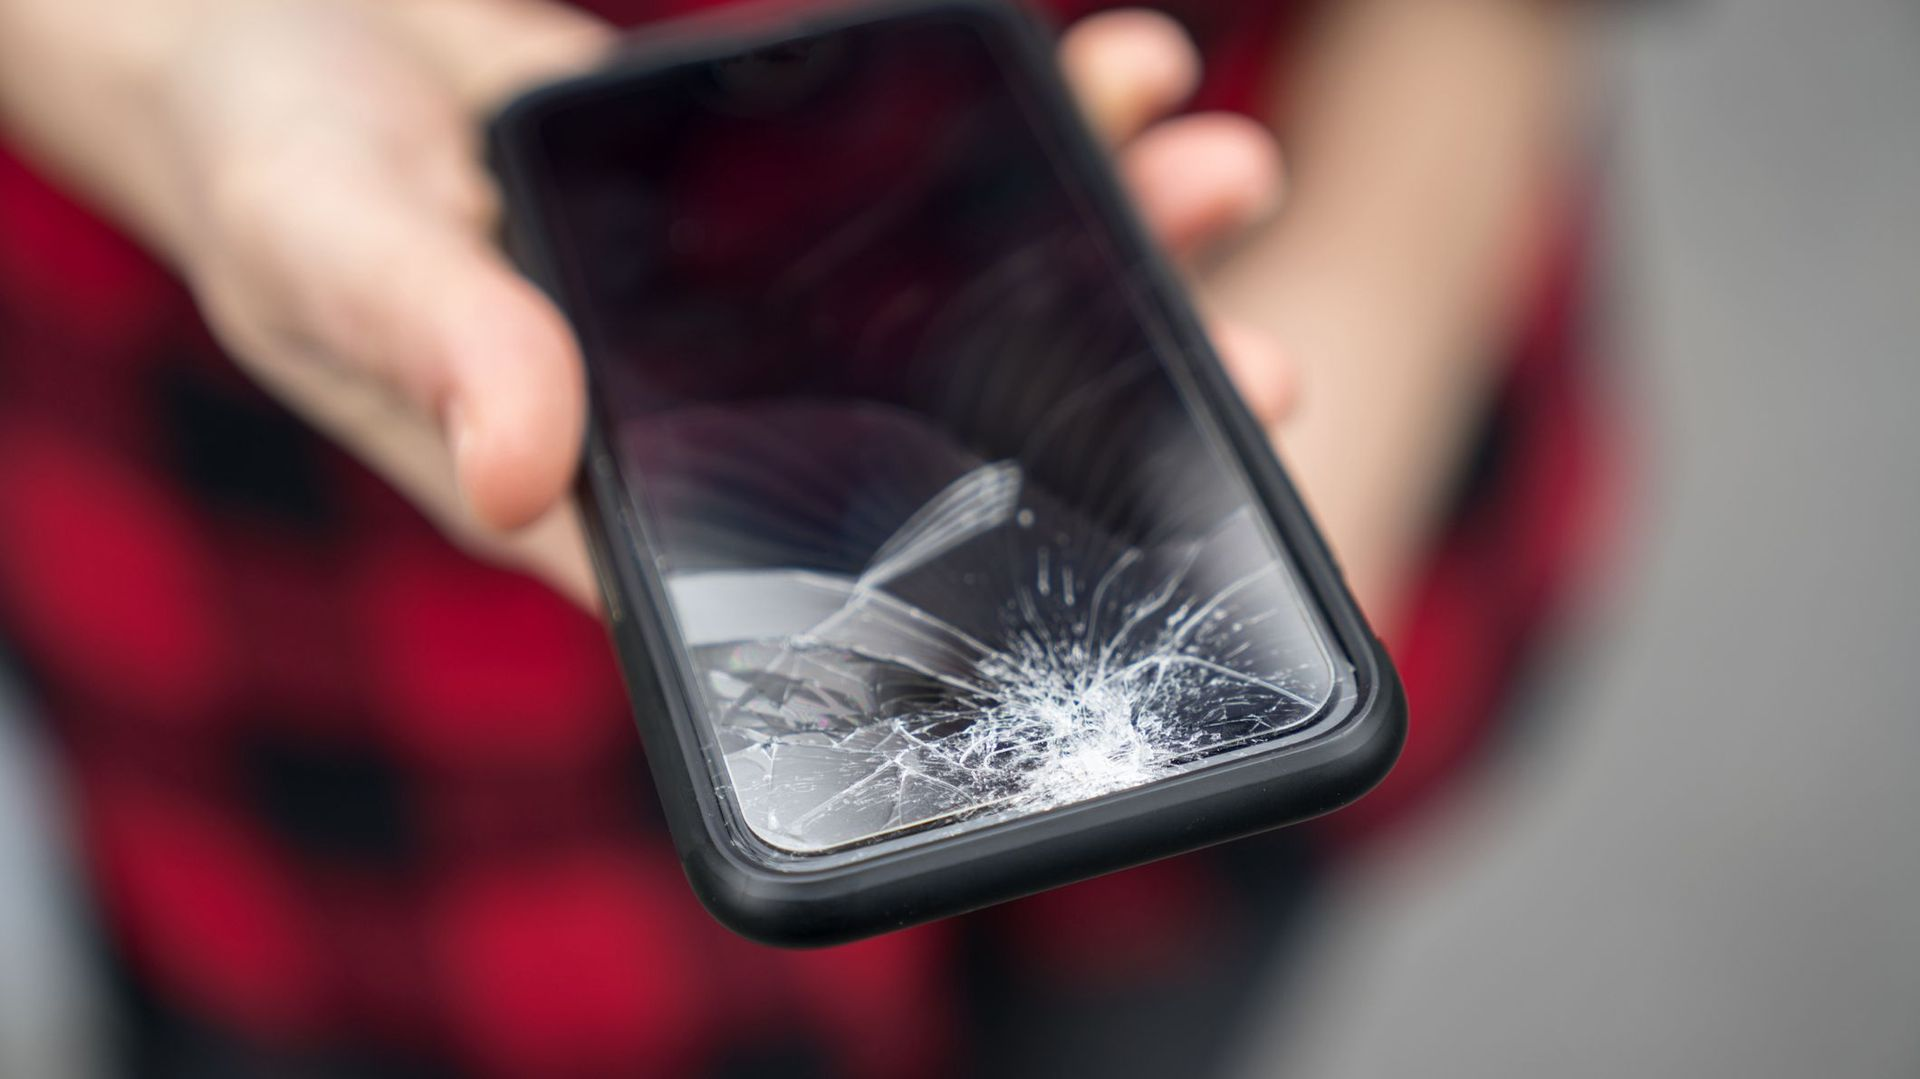
\includegraphics[width=\linewidth]{fc23c2280ceeb0d2edc34ce22218e61e-1540472534.jpg}}{%
      \fbox{\parbox[c][3.5cm][c]{0.9\linewidth}{\centering\footnotesize
      [image : \texttt{fc23\dots.jpg} à téléverser]}}}\\[3pt]
    {\tiny Source : RTBF}
  \column{0.5\textwidth}
    \footnotesize
    \begin{itemize}
      \item Des millions d'écrans se brisent chaque année lors d'une \textbf{chute}.
      \item La fissure s'amorce presque toujours à un \textbf{coin} ou un \textbf{bord}.
      \item \textbf{Idée :} une \textbf{épaisseur variable} du \textbf{verre trempé}
            pourrait-elle réduire ce risque en préservant la \textbf{tactilité} ?
    \end{itemize}
  \end{columns}
\end{frame}

% ============ Problematique ============
\begin{frame}{Problématique}
  \vfill
  \begin{center}
  \begin{beamercolorbox}[wd=0.92\textwidth,sep=14pt,rounded=true,shadow=true]{block body}
  \centering\large
  \textbf{Est-il possible de fabriquer un écran protecteur en verre trempé à
  l'épaisseur \emph{non uniforme}} --- fin au centre, épais aux bords ---
  \textbf{pour réduire la probabilité de rupture}, sans sacrifier la tactilité
  ni la masse ?
  \end{beamercolorbox}
  \end{center}
  \vfill
\end{frame}

% ============ Plan ============
\begin{frame}{Plan}
  \vfill
  \Large
  \begin{enumerate}[leftmargin=2.4em,itemsep=12pt,
                    label=\textcolor{verre}{\bfseries\arabic*.}]
    \item Le \textbf{modèle} utilisé
    \item Les \textbf{paramètres} et les \textbf{lois} utilisées
    \item L'\textbf{étude théorique} des fissures de bords
    \item La \textbf{validation expérimentale}
    \item La \textbf{conclusion}
  \end{enumerate}
  \vfill
\end{frame}


% =====================================================================
\section{Le modèle utilisé}
% =====================================================================
\begin{frame}{1. Le modèle --- hypothèses}
  \footnotesize
  \begin{itemize}
    \item \textbf{Plaque mince réduite à une poutre 1D} : épaisseur
          $e\sim 0{,}5$~mm $\ll$ dimensions $\sim 100$~mm $\Rightarrow$ flexion
          dominante, cisaillement négligé.
    \item \textbf{Élasticité linéaire isotrope} : $E=73$~GPa, $\nu=0{,}22$.
    \item \textbf{Rupture fragile} : pas de plasticité ; rupture si la traction
          de surface dépasse un seuil $\sigma_c$.
    \item \textbf{Précontrainte de compression} (trempe chimique) : élève le
          seuil effectif à $\sigma_c\sim 850$~MPa.
    \item \textbf{Choc traité par l'énergie} : une fraction $\eta\approx 5\%$ de
          l'énergie de chute est stockée en flexion (hypothèse forte, assumée).
  \end{itemize}
  \vspace{2pt}
  \centering\scriptsize\textcolor{danger}{Ces hypothèses rendent le modèle
  \emph{conservatif} : on surestime légèrement la contrainte.}
\end{frame}

% ---- 1.1 la chute ----
\begin{frame}{1.1 La chute : de la hauteur à l'énergie}
  \begin{columns}[c]
  \column{0.42\textwidth}
    \centering
    \begin{tikzpicture}[scale=0.8]
      \draw[-{Latex}](0,4.4)--(0,-0.2);
      \phone{1.4}{3.8}{verre}
      \draw[-{Latex[length=2mm]},danger,thick](1.4,3.0)--(1.4,2.2) node[midway,right,font=\tiny]{$v$};
      \phone{1.4}{0.6}{gristik}
      \sol{0.4}{2.6}
      \draw[{Latex}-{Latex}](0.15,0)--(0.15,3.8) node[midway,left,font=\tiny]{$h$};
    \end{tikzpicture}
  \column{0.58\textwidth}
    \footnotesize
    \[ v=\sqrt{2gh}\,,\qquad E_c=\tfrac12 m v^{2}=mgh \]
    Avec $m=180$~g :
    \begin{center}\scriptsize
    \begin{tabular}{ccc}
    \toprule
    $h$ (m) & $v$ (m/s) & $E_c$ (J) \\
    \midrule
    0,5 & 3,1 & 0,9 \\
    \textbf{1,0} & \textbf{4,4} & \textbf{1,8} \\
    1,5 & 5,4 & 2,7 \\
    2,0 & 6,3 & 3,5 \\
    \bottomrule
    \end{tabular}
    \end{center}
    \textcolor{verre}{Cas de référence : $h=1$~m $\Rightarrow E_c\approx 1{,}8$~J.}
  \end{columns}
\end{frame}

% ---- 1.2 oscillateur ----
\begin{frame}{1.2 Le verre se comporte comme un ressort}
  \begin{columns}[c]
  \column{0.45\textwidth}
    \centering
    \begin{tikzpicture}[scale=0.95]
      \draw[thick](0,-0.2)--(0,1.8);
      \foreach \yy in {-0.1,0.2,...,1.7}{\draw[gristik](0,\yy)--(-0.22,\yy-0.18);}
      \draw[decorate,decoration={coil,aspect=0.6,segment length=4pt,amplitude=4pt},verre,thick](0,0.8)--(2.0,0.8);
      \draw[fill=verre!15,thick](2.0,0.3) rectangle (2.9,1.3);
      \draw[-{Latex},danger,thick](3.0,0.8)--(3.7,0.8) node[right,font=\tiny]{$x$};
    \end{tikzpicture}
  \column{0.55\textwidth}
    \footnotesize Conservation de l'énergie :
    \[ \tfrac12\,k\,x_{\max}^{2}=\eta\,E_c
       \;\Rightarrow\; x_{\max}=\sqrt{\frac{2\eta E_c}{k}} \]
    $k$ : \textbf{raideur} de l'écran, $x_{\max}$ : fléche maximale.\\[4pt]
    \textcolor{danger}{\textbf{Hypothèse :} $\eta\approx 5\%$ (le reste : rebond,
    son, corps du téléphone).}
  \end{columns}
\end{frame}

% ---- 1.3 poutre k ~ e^3 ----
\begin{frame}{1.3 Poutre en flexion : la raideur varie en $e^{3}$}
  \begin{columns}[c]
  \column{0.4\textwidth}
    \centering
    \begin{tikzpicture}[scale=0.95]
      \draw[verre,thick,fill=verre!12](0,0) rectangle (2.2,0.7);
      \draw[{Latex}-{Latex}](0,-0.25)--(2.2,-0.25) node[midway,below,font=\tiny]{$b$};
      \draw[{Latex}-{Latex}](2.45,0)--(2.45,0.7) node[midway,right,font=\tiny]{$e$};
    \end{tikzpicture}
  \column{0.6\textwidth}
    \footnotesize
    \[ I=\frac{b\,e^{3}}{12},\qquad
       k=\frac{48\,E\,I}{L^{3}}=\frac{4Eb}{L^{3}}\,e^{3}
       \;\propto\; e^{3} \]
    Avec $b=20$~mm, $L=50$~mm, $e=0{,}5$~mm :
    \[ k\approx 5{,}8\times10^{3}~\mathrm{N/m},\quad
       x_{\max}\approx 5{,}5~\mathrm{mm}. \]
    \centering\textcolor{verre}{Doubler $e$ $\Rightarrow$ raideur $\times 8$.}
  \end{columns}
\end{frame}

% ---- 1.4 contrainte ----
\begin{frame}{1.4 La loi centrale : $\sigma_{\max}\propto 1/\sqrt{e}$}
  \footnotesize
  Contrainte de flexion (peau tendue) : $\displaystyle \sigma_{\max}=\frac{6\,E\,e}{L^{2}}\,x_{\max}$.
  En remplaçant $x_{\max}=\sqrt{2\eta E_c/k}$ et $k\propto e^{3}$ :
  \[ \boxed{\;\sigma_{\max}=\frac{6Ee}{L^{2}}\sqrt{\frac{2\eta E_c}{k}}
     \;\propto\; \frac{\sqrt{\eta E_c}}{\sqrt{e}}\;\;(\propto e^{-1/2})\;} \]
  \centering Au centre ($L=50$~mm, $h=1$~m) : $\sigma_{\max}\approx 480$~MPa.
\end{frame}

% ---- 1.5 graphe sigma(e) avec valeurs ----
\begin{frame}{1.5 Ordre de grandeur : $\sigma_{\max}(e)$}
  \centering
  \begin{tikzpicture}[scale=1]
    % echelle unique : x_cm = e(mm)*4.5 ; y_cm = sigma(MPa)/200
    \draw[-{Latex}](0,0)--(7.6,0) node[right,font=\scriptsize]{$e$ (mm)};
    \draw[-{Latex}](0,0)--(0,5) node[above,font=\scriptsize]{$\sigma_{\max}$ (MPa)};
    \foreach \e in {0.3,0.5,0.8,1.0,1.5}{
      \draw ({\e*4.5},0)--({\e*4.5},-0.1) node[below,font=\tiny]{\e};}
    \foreach \s/\yc in {300/1.5,500/2.5,700/3.5,900/4.5}{
      \draw (0,\yc)--(-0.1,\yc) node[left,font=\tiny]{\s};}
    \draw[danger,dashed](0,4.25)--(7.2,4.25) node[right,font=\tiny,danger]{seuil $\approx$850};
    \draw[verre,very thick,domain=0.28:1.55,samples=80,smooth]
      plot ({\x*4.5},{482*sqrt(0.5/\x)/200});
    \foreach \e/\s in {0.3/622,0.5/482,1.0/341,1.5/278}{
      \fill[danger] ({\e*4.5},{\s/200}) circle (1.6pt);
      \node[font=\tiny,above right] at ({\e*4.5},{\s/200}){\s};}
  \end{tikzpicture}
  \par\footnotesize Plus l'écran est épais, plus la contrainte chute
  ($\sigma\propto e^{-1/2}$) : tendance qui justifie d'épaissir les zones à risque.
\end{frame}


% =====================================================================
\section{Paramètres et lois}
% =====================================================================
\begin{frame}{2.1 Paramètres du matériau (verre aluminosilicate trempé)}
  \centering\small
  \begin{tabular}{lll}
  \toprule
  Grandeur & Valeur & Source \\
  \midrule
  Module d'Young $E$ & $73$~GPa & Corning \\
  Coefficient de Poisson $\nu$ & $0{,}22$ & Corning \\
  Masse volumique $\rho$ & $2450$~kg/m$^3$ & Corning \\
  Compression de surface (CS) & $700$--$850$~MPa & Gy (2008) \\
  Profondeur de couche (DOL) & $30$--$50~\mu$m & Gy (2008) \\
  \bottomrule
  \end{tabular}
  \vspace{0.4cm}
  \par\footnotesize La \textbf{trempe chimique} (échange ionique
  $\mathrm{K}^{+}/\mathrm{Na}^{+}$) crée une compression de surface : la rupture
  n'apparaît qu'au-delà d'une traction $\sim 850$~MPa.
\end{frame}

\begin{frame}{2.2 Paramètres du modèle}
  \footnotesize
  \begin{columns}[T]
  \column{0.5\textwidth}
    \textbf{Géométrie / chute}
    \begin{itemize}
      \item masse $m=180$~g
      \item hauteur $h\sim 1$~m (loi de tirage)
      \item largeur de bande $b\approx 20$~mm
      \item portée effective $L=25$ à $50$~mm (selon la zone)
    \end{itemize}
  \column{0.5\textwidth}
    \textbf{Énergie / rupture}
    \begin{itemize}
      \item fraction de flexion $\eta\approx 5\%$
      \item seuil $\sigma_c\approx 850\pm120$~MPa
      \item module de Weibull $m_W\approx 8$
    \end{itemize}
  \end{columns}
  \vspace{0.3cm}
  \centering\scriptsize\textcolor{danger}{$\eta$, $b$ et $L$ sont des paramètres
  effectifs calés sur les ordres de grandeur ; ils n'affectent pas le
  \emph{classement} des profils.}
\end{frame}

\begin{frame}{2.3 Loi de rupture fragile (statistique)}
  \begin{columns}[c]
  \column{0.5\textwidth}
    \footnotesize
    Le verre casse de façon \textbf{aléatoire} (micro-défauts). Loi de
    \textbf{Weibull} :
    \[ P_r(\sigma)=1-\exp\!\Big[-\big(\tfrac{\sigma}{\sigma_\theta}\big)^{m_W}\Big] \]
    En pratique : on tire un \textbf{seuil} $\sigma_c$ autour de
    $850$~MPa (écart-type $\sim 120$~MPa).
  \column{0.5\textwidth}
    \centering
    \begin{tikzpicture}[scale=1]
      \draw[-{Latex}](0,0)--(5.2,0) node[right,font=\tiny]{$\sigma_c$ (MPa)};
      \draw[-{Latex}](0,0)--(0,2.6) node[above,font=\tiny]{densité};
      % gaussienne centree 850, x_cm = (sigma-500)/130 ; 850->2.69
      \draw[verre,very thick,domain=520:1200,samples=80,smooth]
        plot ({(\x-500)/130},{2.2*exp(-(\x-850)*(\x-850)/(2*120*120))});
      \draw[danger,dashed](2.69,0)--(2.69,2.2) node[above,font=\tiny,danger]{850};
      \foreach \s in {600,850,1100}{
        \draw ({(\s-500)/130},0)--({(\s-500)/130},-0.1) node[below,font=\tiny]{\s};}
    \end{tikzpicture}
  \end{columns}
\end{frame}

% =====================================================================
\section{Étude théorique des fissures de bords}
% =====================================================================
\begin{frame}{3.1 Pourquoi la fissure part du bord}
  \begin{columns}[c]
  \column{0.5\textwidth}
    \centering
    \begin{tikzpicture}[scale=0.9]
      % centre : grande portee
      \fill[gristik](0,2.2)--(-0.25,1.9)--(0.25,1.9)--cycle;
      \fill[gristik](4,2.2)--(3.75,1.9)--(4.25,1.9)--cycle;
      \draw[verre,very thick](0,2.2) .. controls (2,1.75) .. (4,2.2);
      \draw[-{Latex},danger](2,3)--(2,2.15);
      \draw[{Latex}-{Latex}](4.3,1.9)--(4.3,2.2) node[right,font=\tiny]{$L$ grand};
      % coin : petite portee
      \fill[gristik](0,0.4)--(-0.2,0.15)--(0.2,0.15)--cycle;
      \fill[gristik](1.4,0.4)--(1.2,0.15)--(1.6,0.15)--cycle;
      \draw[danger,very thick](0,0.4) .. controls (0.7,0.0) .. (1.4,0.4);
      \draw[-{Latex},danger](0.7,1.0)--(0.7,0.35);
      \draw[{Latex}-{Latex}](1.7,0.15)--(1.7,0.4) node[right,font=\tiny]{$L$ petit};
    \end{tikzpicture}
  \column{0.5\textwidth}
    \footnotesize
    On montre que $\displaystyle \sigma_{\max}\propto \frac{K_c}{\sqrt{L}}$ :
    \begin{itemize}
      \item au \textbf{coin}, la portée $L$ est petite ;
      \item s'ajoute une \textbf{concentration de contrainte} $K_c\approx 1{,}7$.
    \end{itemize}
    \centering\textcolor{danger}{$\Rightarrow$ contrainte maximale au coin.}
  \end{columns}
\end{frame}

\begin{frame}{3.2 Ordre de grandeur : contrainte par zone ($e=0{,}5$~mm, $h=1$~m)}
  \centering
  \begin{tikzpicture}[scale=1]
    % y_cm = sigma/300 ; seuil 850 -> 2.83 ; coin 1158 -> 3.86
    \draw[-{Latex}](0,0)--(0,4.4) node[above,font=\scriptsize]{$\sigma_{\max}$ (MPa)};
    \draw(0,0)--(6.3,0);
    \foreach \s in {300,600,900,1200}{
      \draw(0,{\s/300})--(-0.1,{\s/300}) node[left,font=\tiny]{\s};}
    \draw[danger,dashed](0,2.83)--(6.3,2.83) node[right,font=\tiny,danger]{seuil 850};
    \fill[verre!70](0.5,0) rectangle (1.7,{482/300});
    \fill[orange!75](2.5,0) rectangle (3.7,{751/300});
    \fill[danger!75](4.5,0) rectangle (5.7,{1158/300});
    \node[font=\tiny] at (1.1,{482/300+0.25}){482};
    \node[font=\tiny] at (3.1,{751/300+0.25}){751};
    \node[font=\tiny] at (5.1,{1158/300+0.25}){1158};
    \node[font=\tiny,below] at (1.1,0){centre};
    \node[font=\tiny,below] at (3.1,0){bord};
    \node[font=\tiny,below] at (5.1,0){coin};
  \end{tikzpicture}
  \par\footnotesize Au \textbf{coin}, $\sigma_{\max}\approx 1160$~MPa
  \textbf{dépasse} le seuil ($850$~MPa) : c'est là que la rupture s'amorce.
\end{frame}

% ---- 3.3 Monte-Carlo principe ----
\begin{frame}{3.3 Quantifier le risque : méthode de Monte-Carlo}
  \footnotesize
  Chaque chute est différente : on en simule un grand nombre au hasard.
  \begin{itemize}[itemsep=3pt]
    \item[\textcolor{verre}{\textbf{1.}}] \textbf{Tirer} une chute (hauteur $h$, angle d'impact).
    \item[\textcolor{verre}{\textbf{2.}}] \textbf{Calculer} $\sigma_{\max}$ (modèle poutre).
    \item[\textcolor{verre}{\textbf{3.}}] \textbf{Comparer} au seuil : casse si $\sigma_{\max}>\sigma_c$.
    \item[\textcolor{verre}{\textbf{4.}}] \textbf{Répéter} $N=5000$ fois.
    \item[\textcolor{verre}{\textbf{5.}}] \textbf{Estimer} $P(\text{rupture})\approx \dfrac{\text{casses}}{N}$.
  \end{itemize}
  \centering\scriptsize Convergence garantie par la \textbf{loi des grands nombres}.
\end{frame}

% ---- 3.4 angle gaussien ----
\begin{frame}{3.4 On tire l'angle selon une loi réaliste}
  \footnotesize Gaussienne $\mu=65^\circ$, $\sigma=15^\circ$, tronquée sur
  $[10^\circ,90^\circ]$ : les grands angles (coin) dominent.
  \vspace{0.1cm}
  \centering
  \begin{tikzpicture}[scale=0.95]
    \draw[-{Latex}](0,0)--(9,0) node[right,font=\scriptsize]{$\theta\,(^\circ)$};
    \draw[-{Latex}](0,0)--(0,3.2) node[above,font=\scriptsize]{densité};
    \draw[verre,very thick,domain=10:90,samples=120,smooth]
      plot ({(\x-10)*8/80},{2.6*exp(-(\x-65)*(\x-65)/450)});
    \draw[danger,dashed](5.5,0)--(5.5,2.6) node[above,font=\scriptsize,danger]{$\mu=65^\circ$};
    \draw[{Latex}-{Latex},ok,thick](5.5,1.1)--(7,1.1) node[midway,above,font=\scriptsize,ok]{$\sigma=15^\circ$};
    \foreach \x/\lab in {0/10,4/50,5.5/65,7/80,8/90}{
      \draw (\x,0)--(\x,-0.12) node[below,font=\tiny]{\lab};}
  \end{tikzpicture}
\end{frame}

% ---- 3.5 resultats P(rupture) ----
\begin{frame}{3.5 Résultat : le profil change tout ($N=5000$)}
  \begin{columns}[c]
  \column{0.55\textwidth}
    \centering
    \begin{tikzpicture}[yscale=0.042,xscale=1.05]
      \draw[-{Latex}](0,0)--(0,70) node[above,font=\scriptsize]{$P$ (\%)};
      \draw(0,0)--(5.1,0);
      \foreach \y in {0,20,40,60}{\draw(0,\y)--(-0.12,\y) node[left,font=\tiny]{\y};}
      \fill[danger!70](0.4,0) rectangle (1.4,59);
      \fill[ok!70](2.0,0) rectangle (3.0,13);
      \fill[verre!70](3.6,0) rectangle (4.6,10);
      \node[font=\tiny] at (0.9,64){59\%};
      \node[font=\tiny] at (2.5,18){13\%};
      \node[font=\tiny] at (4.1,15){10\%};
      \node[font=\tiny,below] at (0.9,0){Uniforme};
      \node[font=\tiny,below] at (2.5,0){Parabol.};
      \node[font=\tiny,below] at (4.1,0){Expon.};
    \end{tikzpicture}
  \column{0.45\textwidth}
    \footnotesize À centre identique ($e_c=0{,}5$~mm), épaissir les bords
    (jusqu'à $e_b=1{,}2$~mm) fait passer le risque de
    \textbf{\textcolor{danger}{59\%}} à
    \textbf{\textcolor{ok}{$\sim$10--13\%}}.\\[3pt]
    \scriptsize (valeurs de simulation, ordres de grandeur)
  \end{columns}
\end{frame}

% ---- 3.6 optimisation ----
\begin{frame}{3.6 Optimisation sous contraintes}
  \begin{columns}[c]
  \column{0.55\textwidth}
    \centering
    \begin{tikzpicture}[scale=0.6]
      \foreach \i in {0,...,5}{\foreach \j in {0,...,3}{
        \pgfmathtruncatemacro\P{55 - \i*9 - \j*2}
        \pgfmathtruncatemacro\g{max(0,min(100,\P*1.6))}
        \fill[red!\g!green!88] (\i,\j) rectangle ++(1,1);
        \node[font=\tiny,white] at (\i+0.5,\j+0.5){\P};}}
      \draw[step=1,gray!60,thin](0,0) grid (6,4);
      \fill[pattern=north east lines,pattern color=black](5,3) rectangle (6,4);
      \node[star,star points=5,star point ratio=2.2,fill=yellow,draw=black,scale=0.7](opt) at (5.5,2.5){};
      \node[font=\tiny,below=1pt of opt]{optimum};
      \foreach \i/\lab in {0/0.5,2/1.1,4/1.7,5/2.0}{\node[font=\tiny,below] at (\i+0.5,0){\lab};}
      \node[font=\scriptsize,below] at (3,-0.55){$e_b$ (mm)};
      \foreach \j/\lab in {0/0.2,2/0.4,3/0.5}{\node[font=\tiny,left] at (0,\j+0.5){\lab};}
      \node[font=\scriptsize,rotate=90] at (-1.0,2){$e_c$ (mm)};
    \end{tikzpicture}
  \column{0.45\textwidth}
    \footnotesize On minimise $P$ sous : \textbf{tactilité} $e_c\le 0{,}5$~mm et
    \textbf{masse} $\le 2{,}5\times$.
    \begin{block}{Optimum}
    \centering\footnotesize centre fin + bords épais ($e_b\approx 2$~mm)
    $\Rightarrow P\approx 3\%$
    \end{block}
    \scriptsize Les deux contraintes sont saturées (chiffres en \% dans la carte).
  \end{columns}
\end{frame}


% =====================================================================
\section{Validation expérimentale}
% =====================================================================
\begin{frame}{4.1 Vérifier la loi avec un circuit électrique}
  \footnotesize
  Mesurer $\sigma$ et $e$ sur du verre est difficile. Mais l'\textbf{oscillateur
  mécanique} et un \textbf{circuit RLC série} obéissent à la même équation : on
  reproduit la dynamique du choc par une \textbf{impulsion électrique} et on
  vérifie $\sigma_{\max}\propto e^{-1/2}$ \textbf{avec des grandeurs électriques}.
  \vspace{0.3cm}
  \centering
  \begin{tikzpicture}[scale=0.9]
    \draw[decorate,decoration={coil,segment length=3pt,amplitude=3pt},verre,thick](0,1.2)--(1.2,1.2);
    \draw[fill=verre!12,thick](1.2,0.9) rectangle (1.9,1.5);
    \node[font=\scriptsize] at (0.95,0.6){ressort + masse};
    \node[font=\scriptsize] at (2.6,1.2){$\equiv$};
    \draw[ok,very thick](3.3,1.35)--(3.9,1.35) (3.3,1.05)--(3.9,1.05);
    \node[font=\scriptsize] at (3.6,0.6){circuit RLC};
  \end{tikzpicture}
\end{frame}

\begin{frame}{4.2 Le dictionnaire de l'analogie}
  \begin{columns}[c]
  \column{0.5\textwidth}
    \centering\footnotesize
    \[ m\ddot{x}+c\dot{x}+kx=F(t) \]
    \[ L\ddot{q}+R\dot{q}+\tfrac{1}{C}q=e(t) \]
    \begin{tabular}{ll}
    \toprule
    Mécanique & Électrique \\
    \midrule
    masse $m$ & inductance $L$ \\
    amortissement $c$ & résistance $R$ \\
    raideur $k$ & $1/C$ \\
    fléche $x$ & charge $q$ \\
    \bottomrule
    \end{tabular}
  \column{0.5\textwidth}
    \footnotesize
    Conséquences directes :
    \begin{itemize}
      \item $k\leftrightarrow 1/C$ et $k\propto e^{3}$
            $\Rightarrow \boxed{e\propto C^{-1/3}}$
      \item fléche $x\leftrightarrow$ charge $q$, lue via
            $q_{\max}=C\,u_{C,\max}$
    \end{itemize}
  \end{columns}
\end{frame}

\begin{frame}{4.3 Le montage}
  \centering
  \begin{tikzpicture}[scale=1.1, every node/.style={font=\scriptsize}]
    \draw[thick] (0,0.7) -- (0,0) -- (4,0);
    \draw[thick] (0,1.3) -- (0,2) -- (0.6,2);
    \draw[thick] (1.6,2) -- (2.2,2);
    \draw[thick] (3.0,2) -- (4,2) -- (4,1.18);
    \draw[thick] (4,0.92) -- (4,0);
    \draw[thick] (0,1) circle (0.3);
    \draw[thick] (-0.12,0.95)--(-0.04,0.95)--(-0.04,1.12)--(0.04,1.12)--(0.04,0.9)--(0.12,0.9);
    \node[left] at (-0.45,1) {GBF};
    \draw[verre,thick,decorate,decoration={coil,segment length=4pt,amplitude=4pt}] (0.6,2) -- (1.6,2);
    \node[verre] at (1.1,2.45) {$L\approx 10$~mH};
    \draw[danger,thick] (2.2,1.8) rectangle (3.0,2.2);
    \node[danger] at (2.6,2.45) {$R$};
    \draw[ok,very thick] (3.65,1.18) -- (4.35,1.18);
    \draw[ok,very thick] (3.65,0.92) -- (4.35,0.92);
    \node[ok,right] at (4.45,1.05) {$C$ : 1--100~nF};
    \draw[gray,dashed] (4.35,1.18) -- (5.2,1.6);
    \draw[gray,dashed] (4.35,0.92) -- (5.2,0.5);
    \draw[thick,rounded corners=2pt] (5.2,0.45) rectangle (6.4,1.65);
    \node at (5.8,1.05) {$u_C(t)$};
    \node at (5.8,1.95) {oscilloscope};
  \end{tikzpicture}
  \par\footnotesize On fixe $L,R$ et l'impulsion ; on fait varier $C$ (image de
  l'épaisseur) et on lit $u_C(t)$.
\end{frame}

\begin{frame}{4.4 Protocole et lecture à l'oscilloscope}
  \begin{columns}[c]
  \column{0.5\textwidth}
    \footnotesize
    \begin{enumerate}
      \item Pour chaque $C_i$ : envoyer l'impulsion, relever $u_{C,\max}$ et la
            pseudo-période $T$.
      \item Calculer $e_i\propto C_i^{-1/3}$, $q_{\max}=C_i\,u_{C,\max}$,
            $\sigma_i\propto e_i\,q_{\max}$.
      \item Tracer $\ln\sigma$ en fonction de $\ln e$.
    \end{enumerate}
    \scriptsize Ordre de grandeur : $T=2\pi\sqrt{LC}\approx 60$~$\mu$s à
    $200$~$\mu$s pour $C=10$ à $100$~nF.
  \column{0.5\textwidth}
    \centering {\scriptsize régime transitoire}
    \begin{tikzpicture}[scale=0.85]
      \draw[-{Latex}](0,0)--(3.6,0) node[right,font=\tiny]{$t$};
      \draw[-{Latex}](0,-1)--(0,1.4) node[above,font=\tiny]{$u_C$};
      \draw[verre,thick,smooth,domain=0:3.3,samples=180]
        plot(\x,{1.1*exp(-0.7*\x)*cos(\x*520)});
      \draw[danger,dashed](0,1.1)--(0.35,1.1) node[right,font=\tiny,danger]{$u_{C,\max}$};
    \end{tikzpicture}
  \end{columns}
\end{frame}

\begin{frame}{4.5 Résultat attendu : la pente $-1/2$}
  \begin{columns}[c]
  \column{0.5\textwidth}
    \centering
    \begin{tikzpicture}[scale=0.95]
      \draw[-{Latex}](0,0)--(4,0) node[right,font=\scriptsize]{$\ln e$};
      \draw[-{Latex}](0,0)--(0,3) node[above,font=\scriptsize]{$\ln \sigma$};
      \draw[verre,very thick](0.4,2.5)--(3.6,0.9);
      \foreach \x/\y in {0.6/2.4,1.2/2.1,1.9/1.75,2.6/1.4,3.3/1.05}{
        \fill[danger](\x,\y) circle (2pt);}
      \node[verre,font=\scriptsize] at (2.5,2.3){pente $\approx -\tfrac12$};
    \end{tikzpicture}
  \column{0.5\textwidth}
    \footnotesize
    \begin{block}{Conclusion de l'expérience}
    Les points $(\ln e,\ln\sigma)$ s'alignent sur une droite de pente
    $\boxed{-\tfrac12}$ : la loi $\sigma_{\max}\propto e^{-1/2}$ est vérifiée,
    \textbf{uniquement avec des mesures électriques}.
    \end{block}
    \scriptsize On valide la \emph{dynamique} du choc, pas le verre lui-même.
  \end{columns}
\end{frame}

% =====================================================================
\section{Conclusion}
% =====================================================================
\begin{frame}{5. Conclusion}
  \begin{columns}[c]
  \column{0.55\textwidth}
    \footnotesize
    \begin{block}{Réponse à la problématique}
    Un profil \textbf{fin au centre, épais aux bords} est physiquement très
    favorable : il fait passer le risque de casse de
    \textcolor{danger}{$\approx 59\%$} (uniforme $0{,}5$~mm) à
    \textcolor{ok}{$\approx 3$--$13\%$}.
    \end{block}
    Tout repose sur une loi simple, démontrée et vérifiée :
    \[ \sigma_{\max}\propto \frac{1}{\sqrt{e}} \]
    obtenue avec \textbf{énergie + poutre}, validée par \textbf{analogie RLC}.
  \column{0.45\textwidth}
    \centering
    \begin{tikzpicture}[scale=0.95]
      \draw[fill=danger!30](0,0) rectangle (0.9,3.0);
      \node[font=\tiny] at (0.45,-0.35){uniforme};
      \node[font=\tiny] at (0.45,-0.65){$59\%$};
      \draw[fill=ok!35](1.8,0) rectangle (2.7,0.5);
      \node[font=\tiny] at (2.25,-0.35){optimisé};
      \node[font=\tiny] at (2.25,-0.65){$\sim$3--13\%};
      \draw[-{Latex},thick](1.0,2.4) .. controls (1.45,2.4) .. (1.7,0.8);
      \node[font=\tiny] at (1.45,2.7){$\div 4$ à $5$};
    \end{tikzpicture}
  \end{columns}
\end{frame}

\begin{frame}{5. Limites et ouvertures}
  \begin{columns}[T]
  \column{0.5\textwidth}
    \footnotesize\textbf{Limites}
    \begin{itemize}\scriptsize
      \item modèle \textbf{1D} (poutre) : surestime un peu $\sigma$ ;
      \item $\eta$, $L$, $\sigma_c$ : paramètres effectifs ;
      \item rupture réelle \textbf{statistique} (Weibull spatial).
    \end{itemize}
  \column{0.5\textwidth}
    \footnotesize\textbf{Fabricabilité / ouvertures}
    \begin{itemize}\scriptsize
      \item gradient continu difficile $\Rightarrow$ profil \textbf{en paliers} ;
      \item \textbf{trempe différentielle} aux bords (masse constante) ;
      \item matériaux à \textbf{gradient de propriétés} (FGM).
    \end{itemize}
  \end{columns}
  \vspace{0.5cm}
  \centering\footnotesize \textbf{Sources :} Timoshenko (RDM) ; Feynman
  (oscillations, analogie RLC) ; Weibull (1951) ; Gy (2008) ; Corning ;
  Dunn \& Shultis (Monte-Carlo).
  \vspace{0.3cm}
  \par\centering\Large\textcolor{verre}{Merci de votre attention.}
\end{frame}

\end{document}
